\graphicspath{{./figures}}

\section{Ground Station PCB}
\subsection{Circuit Design}
Since the ground station mainly consists of various sub-systems and components, "typical application" circuits found in component datasheets were mostly employed. The final schematic is found in Appendix \ref{sec:appendix_gs_schematics}.

\subsubsection{Power}
Current calculations should be done to ensure that the voltage regulators and the boost converters can provide enough power where necessary. A car socket can supply up to 10 A at +12 V (i.e. 120 W). The supply voltage, current consumption, and power consumption of the various system components is listed in Table \ref{tab:gs_component_consumption}. In all cases, maximum current is provided.

\begin{table}[!htb]
  \centering
  \renewcommand{\arraystretch}{1.2}
  \begin{tabular}{ |c|c|c|c| }
  \hline
  \textbf{Component}        & \textbf{Voltage}    & \textbf{Current}     & \textbf{Power}   \\
  \hline
  Motors                    & 24 V                & 0.5 A (x4)           & 48 W             \\ \hline
  ESP32 Dev Board           & 5 V                 & 120 mA               & 660 mW           \\ \hline
  RA-02                     & 3.3 V               & 100 mA               & 330 mW           \\ \hline
  ATGM332D-5N31             & 3.3 V               & 25 mA                & 82.5 mW          \\ \hline
  MPU-9250                  & 3.3 V               & 3.7 mA               & 12.21 mW         \\ \hline
  \end{tabular}
  \caption{Ground Station Component Power Consumption}
  \label{tab:gs_component_consumption}
\end{table}

Therefore, maximum consumption - even at full motor current draw - is only 50 W, and will not place heavy load on the car socket battery supply. The 3.3 V regulator should be able to supply around 130 mA, and the 5 V regulator around $\SI{120}{mA} + (\SI{130}{mA} \times \frac{\SI{3.3}{V}}{\SI{5}{V}}) \approx \SI{210}{mA}$. The LD1117CV can supply up to $\SI{800}{mA}$, and the L7805CP up to $\SI{1.5}{A}$, meaning the limitations are met.

The power section also includes selector jumpers to isolate it from the rest of the board. In this way, if a component is damaged during implementation, or if the power section is found to not be working, external power can be supplied appropriately.

\subsubsection{Motor Drivers}
The L6219 drivers require a reference voltage to set the maximum current. According to the datasheet \cite{datasheet-L6219}, a peak current of $I_{max} = 10 \times \frac{V_{ref}}{R_s}$ in mA is used. Since the recommended value of $R_s = \SI{1}{\ohm}$ is being used, $I_{max} = 10 \times V_{ref}$ mA. Since the motors allow up to 500 mA per winding, a current value of $I_{max} = \SI{475}{mA}$ is chosen to prevent damaging the motors. Therefore, $V_{ref} = \SI{4.75}{V}$. This can be implemented with a voltage divider. Setting the upper resistor $R_1 = \SI{1}{\kilo \ohm}$ results in $R_2 \approx \SI{20}{\kilo \ohm}$, as shown in the schematic. The disadvantage of this method is that the maximum current cannot be controlled dynamically. The reference voltage can be replaced with a DAC from the MCU if more control is required.

\subsubsection{Connectors}
The RA-02 RF module states that not all data pins are necessary. A connector is provided for unused GPIO pins, the SPI, and the unused RF module pins, to allow for flexibility once the PCB is manufactured.

\subsection{PCB Design}
\subsubsection{Stackup}
A 2-layer stackup was decided on, so that the board could be manufactured in-house early on in the project (as the in-house PCB machine has a 2-layer limitation).

\subsubsection{Final Design}
\begin{figure}[!htb]
  \centering
  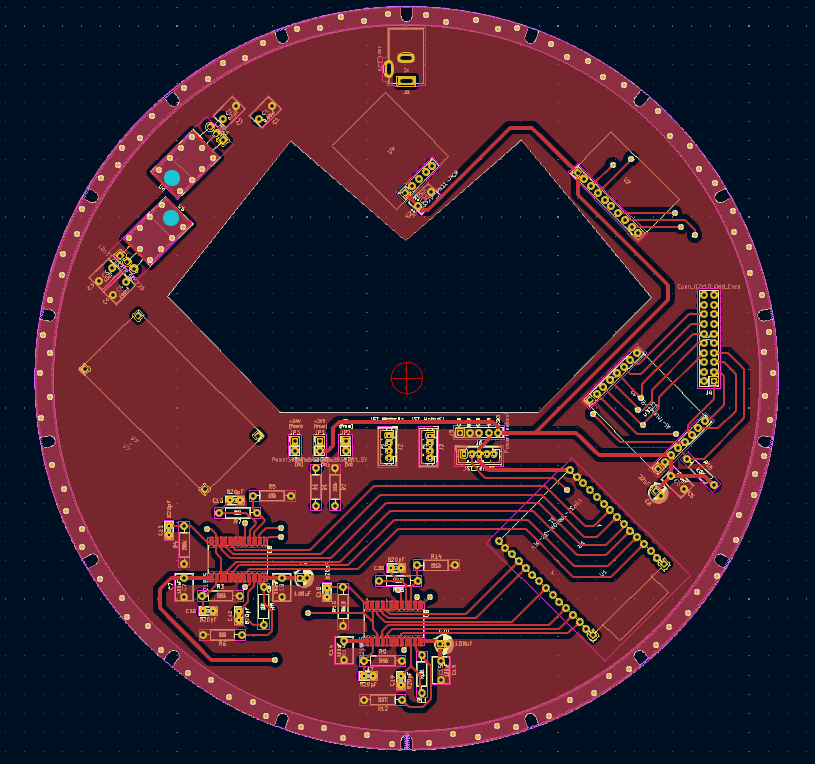
\includegraphics[width=0.6\textwidth]{gs_pcb_design}
  \caption{Ground Station PCB Design}
  \label{fig:gs_pcb}
\end{figure}
The final PCB was designed in KiCAD. It was designed to have a compatible form factor as the previous antenna mount PCB i.e. with a 198 mm outer diameter, outer mounting holes, and holes for the stepper motors. The front layer of this design is shown in Figure \ref{fig:gs_pcb}. Female headers were used for most of the modules, since development boards were being used. Two PCB pours were exposed below the voltage regulators for added heat dissipation.